\section{Results}
\label{sec:results}

\benchmark{} is difficult for the models in our evaluation panel. \figref{fig:model-accuracy} gives the baseline profile: the highest \bsexact{} score is 46\%, strict document-grounded end-to-end accuracy remains low, and the best entry-level accounting scores are much higher than the final balance-sheet scores. JSON formatting is therefore not the main bottleneck. Models often identify numerically plausible postings, but they lose correctness when those local decisions must be tied back to documents and aggregated into the final statement.

\begin{figure*}[t]
\centering
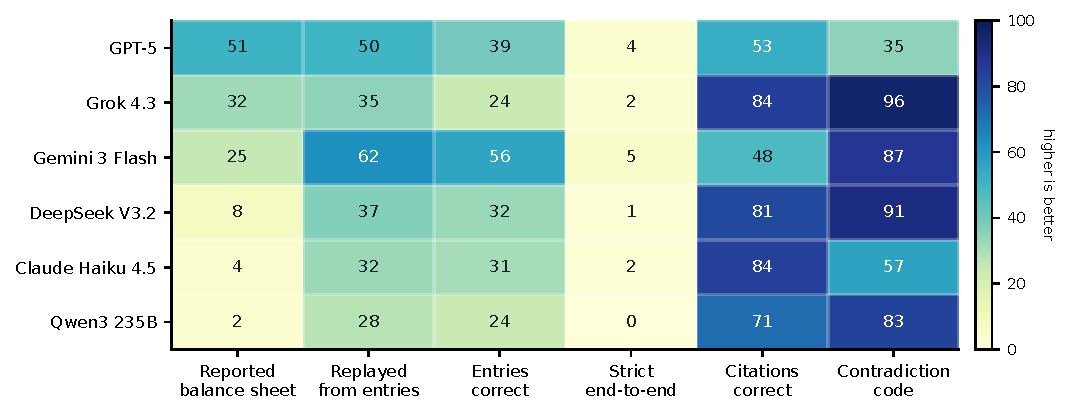
\includegraphics[width=0.92\textwidth]{figures/fig_model_accuracy.pdf}
\caption{Baseline model profile on the 710-record core evaluation split. Balance-sheet and entry metrics use the 480 standard records. \emph{Contradiction code} uses the 230 forced-inconsistency records. \emph{Reported balance sheet} is \bsexact{}. \emph{Replayed from entries} is \bsrecon{}, the balance sheet implied by the model's own journal entries. \emph{Entries correct} ignores document citations. \emph{Strict end-to-end} requires the balance sheet, entries, and citations to match. \emph{Citations correct} is one minus document-reference mismatch incidence per expected posting.}
\label{fig:model-accuracy}
\end{figure*}

The central pattern in \figref{fig:model-accuracy} is the gap between \bsexact{} and \bsrecon{}, where \bsrecon{} parses the model's journal entries, applies them to the opening balance with our ledger, and checks the resulting balance sheet against ground truth. In four of six models the two metrics disagree dramatically: DeepSeek Chat reaches $0.473$ \bsrecon{} but only $0.067$ \bsexact{}, a $40.6$\,pp \aggGap{}. Gemini~3 Flash ($+31.3$\,pp), Qwen~3 235B ($+29.0$\,pp), and Claude Haiku~4.5 ($+26.3$\,pp) show the same pattern. Because \bsrecon{} ignores document support, the metric alone cannot establish audit-grounded entries. The observed gap shows that models often recover plausible entries, fail to bind them to evidence, and then fail to aggregate them into an internally consistent reported statement. GPT-5 is comparatively internally consistent ($46.5\%$ \bsexact{}, $46.3\%$ \bsrecon{}), while Grok-4.3 has a smaller gap but lower entry recall (\secref{sec:analysis}).

GPT-5 and Grok-4.3 used reasoning in the headline panel. Compact-split controls associate reasoning with a smaller gap. Switching from DeepSeek Chat to DeepSeek Reasoner raises \bsexact{} from $8.3\%$ to $54.2\%$ and shrinks the gap from $42.0$ to $1.7$\,pp. Higher-reasoning Haiku and Qwen configurations move in the same direction, while disabling Grok reasoning creates a $27.5$\,pp gap. Strict accuracy remains $0$--$4.2\%$ across these controls, and inconsistency-code effects are mixed. Improved aggregation consistency therefore does not yield evidence-grounded reconciliation (\appref{appx:reasoning-controls}).

To test whether the gap reflects aggregation errors beyond entry errors, we apply the model's own entries through the ledger. In this feedback condition (\secref{sec:verifier}), the ledger returns the full balance sheet implied by the model's entries, account-level and total deltas against its reported balance sheet, and one revision turn. \figref{fig:verifier-effects} shows that \bsexact{} gains $+30$ to $+33$\,pp across three model families with a large gap, all significant at $95\%$ paired bootstrap. The estimate compares an independent same-model baseline with the feedback condition. Feedback contains only replayed balances and deltas, without ground-truth values or entry-correctness hints.

Ledger feedback also reduces inconsistency-code accuracy. On the compact ablation split (\figref{fig:verifier-effects}, right), Gemini~3 Flash loses $13.0$\,pp (95\% CI $[-30.4,+4.3]$, not significant), whereas Qwen~3 235B loses $17.4$\,pp (95\% CI $[-34.8,-4.3]$) and Claude Haiku~4.5 loses $52.2$\,pp (95\% CI $[-73.9,-30.4]$). Ledger feedback may focus revisions on reconciling the bundle instead of reconsidering its consistency. A targeted causal test is needed to distinguish this mechanism.

Tool use depends strongly on the interface. Under the prompt-described protocol, models were instructed to request tools by emitting JSON, but none produced an executable call across $572$ compact-split model-record evaluations. When the same tools were exposed through provider-native function calling, models invoked them on $141/143$ Gemini~3 Flash, $134/143$ DeepSeek Chat, $56/143$ GPT-5, and $140/143$ Claude Haiku~4.5 records. Native \bsexact{} is $52.5\%$, $45.8\%$, $52.5\%$, and $23.3\%$, respectively, but strict end-to-end accuracy remains only $3.3$--$5.8\%$. Native tools recover much of the aggregation component when invoked, but strict grounding remains low (\apptabref{tab:native-tools}).

\begin{figure*}[t]
\centering
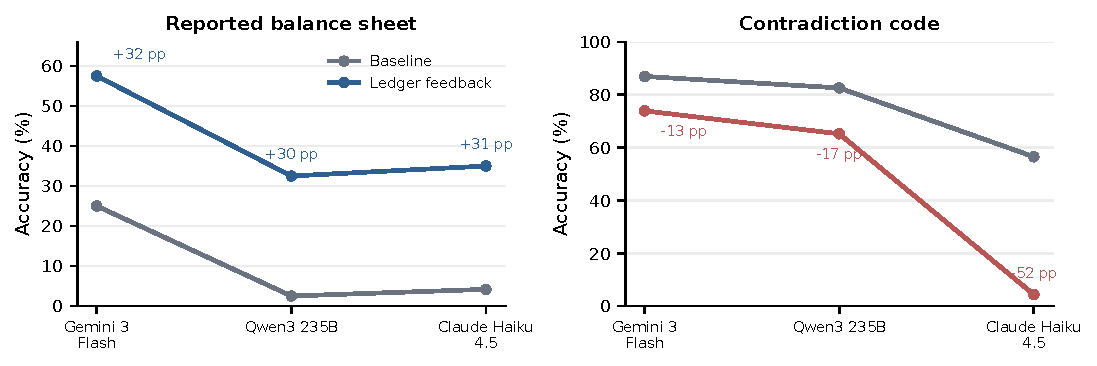
\includegraphics[width=0.98\textwidth]{figures/fig_results_heatmap.pdf}
\caption{One-pass ledger-feedback effect on the compact ablation split ($n{=}143$ per model, with \bsexact{} over $n{=}120$ standard records and \incCode{} over $n{=}23$ forced-inconsistency records). Lines compare each model's independent baseline with the same model after feedback. Labels are percentage-point changes. The tool strongly improves reported balance-sheet accuracy (left) but can reduce contradiction-code accuracy (right). GPT-5 and Grok-4.3 are omitted because they do not exhibit the same aggregation-gap mechanism (\tabref{tab:no-gap-mechanism}).}
\label{fig:verifier-effects}
\end{figure*}

Document linking is the second major failure mode. On the compact split, document-reference mismatches affect $52.4\%$ of expected postings under the greedy matcher, collapsing strict joint accuracy to $5\%$ despite $57\%$ entry-match when citations are ignored. Citation-pressure prompting changes this incidence by only $-1.4$\,pp (CI $[-2.9, 0.0]$), while the \emph{evidence-only} condition lowers it by $-26.4$\,pp (CI $[-29.8, -23.0]$). This contrast locates the main failure in selecting supporting documents instead of following citation instructions (\figref{fig:doc-refs-persistence}).

The primary citation score requires the exact reference set, so we also report a superset-tolerant sensitivity score. Of mismatch postings, $42.0\%$ for Gemini~3 Flash and $58.8\%$ for GPT-5 contain every expected reference plus extras, and $94$--$96\%$ of those extra citations are support documents. Under the sensitivity score, strict end-to-end accuracy rises to $8.8\%$ and $15.8\%$, respectively, but remains low. DeepSeek Chat changes from $2.5\%$ to $3.3\%$ (\appref{appx:citation-sensitivity}).

The uncorrupted templated-text setting isolates accounting reasoning from OCR and layout errors. Seeded substitutions, deletions, token splits, and token merges at achieved character-edit rates of $0.94\%$, $2.20\%$, and $4.45\%$ reduce \bsrecon{} monotonically: Gemini~3 Flash falls from $61.7\%$ uncorrupted to $49.2\%$, and DeepSeek Chat from $50.0\%$ to $36.7\%$. Parse success remains $99$--$100\%$. This control covers character corruption of templated text and excludes raw OCR output and document layout (\appref{appx:ocr-noise}).

\begin{figure}[t]
\centering
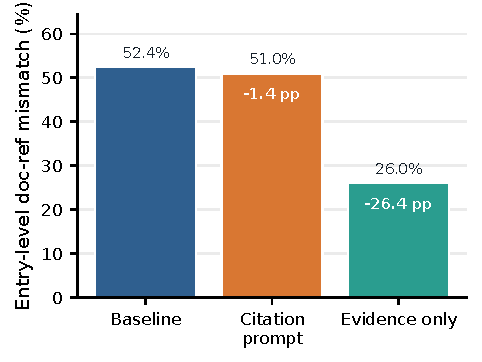
\includegraphics[width=\linewidth]{figures/fig_doc_refs_persistence.pdf}
\caption{Document-linking failure on Gemini~3 Flash over the compact split ($n{=}143$, with the posting metric over $n{=}120$ standard records) persists under explicit citation pressure but drops under the evidence-only condition.}
\label{fig:doc-refs-persistence}
\end{figure}

We also test selection among multiple candidates. On the 45 standard records where Gemini's entries replay to the correct balance sheet but its reported balance sheet is wrong, a ledger-aware best-of-3 selector raises \bsexact{} from $0\%$ to $28.9\%$ (CI $[15.6,42.2]$), while one ledger-feedback revision reaches $84.4\%$ (CI $[73.3,93.3]$). Candidate selection recovers part of the gap. Revision after structured ledger feedback recovers much more (\appfigref{fig:gap-repair}).

\tabref{tab:ablation-summary} distills the ablation results by diagnostic question. Forced ledger-feedback variants produce the only substantial upward movement in \bsexact{}. Removing scaffolding (allowed accounts and support documents) is the most damaging ablation. Prompt-only variants, including a stronger citation instruction and a guided solve protocol, leave the large effects above unchanged. The full primary-model delta plot is in \appfigref{fig:ablation-deltas}.

\begin{table}[t]
\centering
\footnotesize
\setlength{\tabcolsep}{2.4pt}
\renewcommand{\arraystretch}{1.08}
\begin{tabularx}{\linewidth}{@{}p{1.7cm}p{2.55cm}X@{}}
\toprule
Question & Main effect & Interpretation \\
\midrule
Prompt & Guided/self-check prompts change \bsexact{} by at most $2.5$\,pp. Citation pressure changes ref mismatch by $-1.4$\,pp. & Failures primarily reflect mechanisms beyond prompt compliance. \\
Evidence & Removing accounts drops \bsrecon{} by $47.5$\,pp. Removing support documents drops it by $38.3$\,pp. & Account taxonomy and support evidence are essential. \\
Grounding & Evidence-only visibility lowers ref mismatch by $26.4$\,pp. & Evidence selection drives citation failure. \\
Context & Adding 5/15/30 distractors to evidence-only visibility costs $6.7/5.8/8.3$\,pp \bsrecon{}. & Longer context explains part of the task difficulty. \\
Repair & One ledger-feedback turn raises \bsexact{} by $32.5$\,pp on Gemini. Best-of-3 raises it by $28.9$\,pp on the targeted subset. & Global ledger checks repair many reported balance sheets. \\
\bottomrule
\end{tabularx}
\caption{Compact-split ablation summary for Gemini~3 Flash ($n{=}143$, with balance-sheet metrics over $n{=}120$ standard records). Deltas are percentage points against the matched baseline unless a targeted subset is stated.}
\label{tab:ablation-summary}
\end{table}

\begin{figure}[t]
\centering
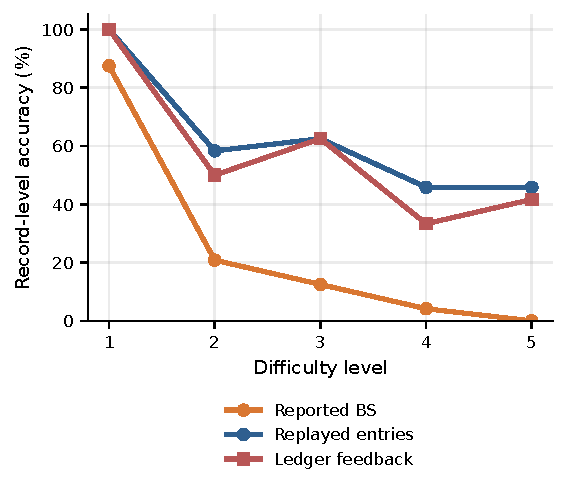
\includegraphics[width=\linewidth]{figures/fig_difficulty_trend.pdf}
\caption{Accuracy by difficulty level for Gemini~3 Flash on the compact split ($n{=}143$, with $24$ standard records per level). As records move from L1 to L5, \bsexact{} collapses much more sharply than the context-stress penalty in \figref{fig:context-stress}. \bsrecon{} remains higher, showing that entry replay remains easier than reporting the final balance sheet.}
\label{fig:difficulty-trend}
\end{figure}

\figrefs{fig:difficulty-trend}{fig:context-stress} compare context length with accounting-logic difficulty. Difficulty produces the larger effect: baseline \bsexact{} falls from $88\%$ at L1 to $0\%$ at L5, while \bsrecon{} declines from $100\%$ to $46\%$. Adding $5$, $15$, or $30$ distractors to an evidence-only document bundle decreases \bsrecon{} by $6.7$, $5.8$, and $8.3$\,pp, respectively. Context accounts for part of the degradation. Accounting dependencies and document choice remain binding even when context is controlled.

\begin{figure}[t]
\centering
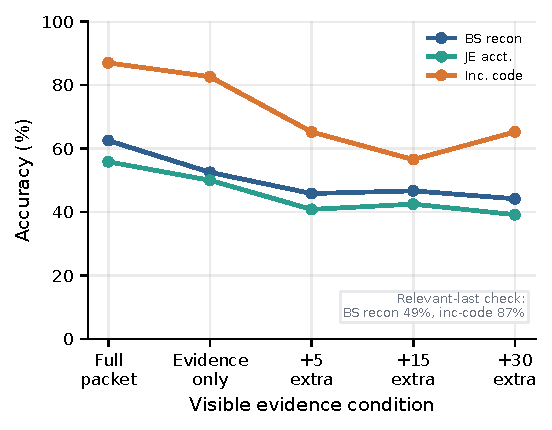
\includegraphics[width=\linewidth]{figures/fig_context_stress.pdf}
\caption{Context stress for Gemini~3 Flash on the compact standard-record split ($n{=}120$), designed to separate longer-context effects from the underlying accounting-logic difficulty. The task remains difficult under controlled evidence. Distractors hurt most when first introduced and then saturate.}
\label{fig:context-stress}
\end{figure}
